\chapter{Models}
After extracting the features, I trained several models to predict the total reading time for each word.

\section{Metrics}
In order to evaluate the performance of the models, I used the following metrics:
\begin{enumerate}
    \item \textbf{Mean Squared Error (MSE)}: This metric measures the average of the squares of the errors, which is the average squared difference between the predicted and actual values. It is calculated as:
    \begin{equation}
        \text{MSE} = \frac{1}{n} \sum_{i=1}^{n} (y_i - \hat{y}_i)^2
    \end{equation}
    where \( n \) is the number of samples, \( y_i \) is the actual value, and \( \hat{y}_i \) is the predicted value. A lower MSE indicates better model performance. The MSE is sensitive to outliers, as it squares the errors, which means that larger errors have a disproportionately large impact on the MSE.

    \item \textbf{R2 Score (Coefficient of Determination)}: This metric measures the proportion of the variance in the dependent variable that is predictable from the independent variables. It is calculated as:
    \begin{equation}
        R^2 = 1 - \frac{\sum_{i=1}^{n} (y_i - \hat{y}_i)^2}{\sum_{i=1}^{n} (y_i - \bar{y})^2}
    \end{equation}
    where \( \bar{y} \) is the mean of the actual values. The R2 score ranges from 0 to 1, where 1 indicates that the model perfectly predicts the dependent variable, and 0 indicates that the model does not explain any of the variance in the dependent variable. A negative R2 score indicates that the model is worse than simply predicting the mean of the dependent variable.

    \item \textbf{Pearson Correlation Coefficient (r)}: This metric measures the linear correlation between the predicted and actual values. It is calculated as:
    \begin{equation}
        r = \frac{\text{cov}(y, \hat{y})}{\sigma_y \sigma_{\hat{y}}}
    \end{equation}
    where \( \text{cov}(y, \hat{y}) \) is the covariance between the actual and predicted values, and \( \sigma_y \) and \( \sigma_{\hat{y}} \) are the standard deviations of the actual and predicted values, respectively. The Pearson correlation coefficient ranges from -1 to 1, where 1 indicates a perfect positive linear correlation, -1 indicates a perfect negative linear correlation, and 0 indicates no linear correlation. A higher absolute value of the Pearson correlation coefficient indicates a stronger linear relationship between the predicted and actual values.

    \item \textbf{Spearman Rank Correlation Coefficient ($\rho$):} This metric measures the strength and direction of the monotonic relationship between the predicted and actual values. It is calculated as the Pearson correlation coefficient of the ranked values. The Spearman rank correlation coefficient ranges from $-1$ to $1$, where $1$ indicates a perfect positive monotonic relationship, $-1$ indicates a perfect negative monotonic relationship, and $0$ indicates no monotonic relationship. It is less sensitive to outliers than the Pearson correlation coefficient.
    
    \item \textbf{Accuracy}: This metric provides an intuitive interpretation of model performance by directly reflecting the average deviation from the true values on a 0–100 scale and it is taken from the \textit{Multilingual Language Models Predict Human Reading Behavior} \cite{hollenstein-etal-2021-multilingual} paper. It is defined as:
    \begin{equation}
        \text{Accuracy} = 100 - \frac{1}{n} \sum_{i=1}^{n} |y_i - \hat{y}_i|
    \end{equation}
    where \( n \) is the number of samples, \( y_i \) is the actual value, and \( \hat{y}_i \) is the predicted value. This is equivalent to subtracting the Mean Absolute Error (MAE) from 100. Since the target values (reading times) are scaled to lie within the range \([0, 100]\), this metric provides a straightforward percentage-based measure of predictive accuracy, where higher values indicate better performance.
\end{enumerate}


\section{Simple Models}

\subsection{Features}
The next step is to extract features from the text that can be used to predict the TRT for each word. I extracted both simple and more complex features. The word features are as follows:

\begin{enumerate}
    \item \textbf{Length:} The number of characters in the word. This feature is simple but effective, as longer words tend to take more time to read.
    
    \item \textbf{Number of tokens:} The number of tokens the word is tokenized into. This feature is useful because the more tokens the word is split into, the longer and more complex it is.
    
    \item \textbf{Frequency:} The frequency of the word in the text. This feature is useful because more frequent words tend to be easier to read and process.
    
    \item \textbf{Surprisal:} The surprisal of the word in the context of the sentence. Surprisal is a measure of how unexpected a word is in a given context, and it is calculated using a language model. I used a pre-trained AutoModelForMaskedLM, \textit{dumitrescustefan/bert-base-romanian-cased-v1}, to calculate the surprisal of each word in the sentence. The surprisal is calculated as the negative logarithm of the probability of the word given the context, which is the sentence in which the word appears. The lower the surprisal, the more predictable the word is in that context.
    
    \item \textbf{Transformer embeddings:} The contextual embedding of the word in the sentence, obtained using a pre-trained transformer model. I used a pre-trained BERT model, \textit{dumitrescustefan/bert-base-romanian-cased-v1}, to obtain the contextual embeddings of each word in the sentence. To make this process more efficient, I first computed the embeddings for each sentence by feeding them through the BERT model and extracting the hidden states from various layers (first, middle, last, and the average across all layers).

    After obtaining the token-level embeddings, I mapped them back to words. Since some words are split into multiple subword tokens by the tokenizer, I averaged the embeddings of all the tokens corresponding to a single word. This mapping was based on character-level offset information provided by the tokenizer. Subword tokens that belong to the same word have contiguous or overlapping character offsets, whereas tokens belonging to different words have non-overlapping offsets. Using this strategy, I reconstructed word-level embeddings from the token embeddings. In the end, I obtained four embeddings for each word: one from the first layer, one from the middle layer, one from the last layer, and one averaged across all layers.
\end{enumerate}

After computing the features for each word, I calculated the Pearson correlation between the features and the total reading time. The results are shown in Table \ref{tab:feature_correlation}. As expected, the length of the word has the highest positive correlation with the TRT, followed by the surprisal and the number of tokens, while the frequency has a similar negative correlation with the TRT. The Pearson correlation is a measure of the linear relationship between two variables, and it ranges from -1 to 1, where -1 indicates a perfect negative correlation, 0 indicates no correlation, and 1 indicates a perfect positive correlation. It is calculated as the covariance of the two variables divided by the product of their standard deviations by the formula:
\begin{equation}
    r = \frac{\text{cov}(X, Y)}{\sigma_X \sigma_Y}
\end{equation}
where \( r \) is the Pearson correlation coefficient, \( X \) and \( Y \) are the two variables, \( \text{cov}(X, Y) \) is the covariance between \( X \) and \( Y \), and \( \sigma_X \) and \( \sigma_Y \) are the standard deviations of \( X \) and \( Y \), respectively.

\begin{table}
    \centering
    \begin{tabular}{|l|c|}
        \hline
        Feature & Correlation with TRT \\
        \hline
        Length & 0.62 \\
        Number of tokens & 0.32 \\
        Frequency & -0.38 \\
        Surprisal & 0.36 \\
        \hline
    \end{tabular}
    \caption{Correlation between features and total reading time (TRT).}
    \label{tab:feature_correlation}
\end{table}

\subsection{Data Preparation}
First, I prepared the data for training the models. I used the features described in the previous chapter and the total reading time for each word as the target. I split the data into train and test sets, with 80\% of the data used for training and 20\% for testing, which means 3796 words for training and 949 words for testing. I also standardized the features using the StandardScaler from scikit-learn, which scales the features to have zero mean and unit variance, then I also standardized the total reading time.

\subsection{Models and Results}
The first models I tried were rather simple ones. I used the scikit-learn library to implement all the models except for the custom neural network, which I implemented using PyTorch.
I trained the models first on the non-embedding features, then on the embeddings, and finally on both the non-embedding features and the embeddings together. The non-embedding features are the length of the word, the number of tokens, the frequency, and the surprisal. The embeddings are the contextual embeddings obtained from the BERT model. The results of the models are shown in Tables \ref{tab:simple_models_results_no_embeddings}, \ref{tab:simple_models_results_embeddings}, and \ref{tab:simple_models_results_all}. Some intuitive plots are found in Figure \ref{fig:simple_models_barplots}. All metrics are computed on the standardized reading times except the accuracy, which is calculated on the reading times in the \([0, 100]\) interval. I tried various hyperparameters for each model and selected the best ones based on the test set performance. The hyperparameters for each model are available in the annex.

\begin{table}[ht]
    \centering
    \caption{Results of simple models trained on different feature sets.}
    \label{tab:simple_models_results}

    \begin{subtable}[t]{\textwidth}
        \centering
        \begin{tabular}{|l|c|c|c|c|c|}
            \hline
            Model & MSE & $R^2$ & Pearson & Spearman & Accuracy \\
            \hline
            Linear Regression                & 0.59 & 0.40 & 0.64 & 0.70 & 93.61 \\
            Elastic Net                      & 0.59 & 0.40 & 0.64 & 0.70 & 93.59 \\
            SGD Regressor                    & 0.59 & 0.40 & 0.64 & 0.70 & 93.65 \\
            Bayesian Ridge                   & 0.59 & 0.40 & 0.64 & 0.70 & 93.61 \\
            SVR Linear Kernel                & 0.63 & 0.37 & 0.63 & 0.70 & 93.34 \\
            SVR RBF Kernel                   & 0.63 & 0.37 & 0.63 & 0.70 & 86.52 \\
            K Neighbors Regressor            & 0.69 & 0.30 & 0.57 & 0.65 & 88.59 \\
            Random Forest Regressor          & 0.63 & 0.36 & 0.63 & 0.67 & 93.32 \\
            Gradient Boosting Regressor      & 0.55 & 0.44 & 0.67 & 0.71 & 93.76 \\
            Hist Gradient Boosting Regressor & 0.57 & 0.43 & 0.66 & 0.71 & 90.13 \\
            Kernel Ridge Linear Kernel       & 0.59 & 0.40 & 0.64 & 0.70 & 93.61 \\
            Kernel Ridge RBF Kernel          & 0.59 & 0.41 & 0.64 & 0.70 & 87.42 \\
            MLP Regressor                    & 0.62 & 0.38 & 0.62 & 0.70 & 93.67 \\
            Custom Neural Network            & 0.60 & 0.37 & 0.63 & 0.68 & 93.57 \\
            \hline
        \end{tabular}
        \caption{Scalar features.}
        \label{tab:simple_models_results_no_embeddings}
    \end{subtable}      
    
    \begin{subtable}[t]{\textwidth}
        \centering
        \begin{tabular}{|l|c|c|c|c|c|}
            \hline
            Model & MSE & $R^2$ & Pearson & Spearman & Accuracy \\
            \hline
            Linear Regression                & 0.65 & 0.34 & 0.61 & 0.66 & 74.29 \\
            Elastic Net                      & 0.60 & 0.39 & 0.63 & 0.70 & 72.73 \\
            SGD Regressor                    & 0.72 & 0.27 & 0.58 & 0.63 & 72.90 \\
            Bayesian Ridge                   & 0.59 & 0.41 & 0.64 & 0.70 & 74.25 \\
            SVR Linear Kernel                & 0.66 & 0.30 & 0.57 & 0.64 & 70.27 \\
            SVR RBF Kernel                   & 0.57 & 0.42 & 0.66 & 0.72 & 74.08 \\
            K Neighbors Regressor            & 0.69 & 0.31 & 0.59 & 0.66 & 75.26 \\
            Random Forest Regressor          & 0.68 & 0.32 & 0.57 & 0.66 & 79.03 \\
            Gradient Boosting Regressor      & 0.67 & 0.32 & 0.58 & 0.65 & 71.49 \\
            Hist Gradient Boosting Regressor & 0.63 & 0.36 & 0.61 & 0.67 & 69.28 \\
            Kernel Ridge Linear Kernel       & 0.65 & 0.34 & 0.61 & 0.66 & 74.32 \\
            Kernel Ridge RBF Kernel          & 0.54 & 0.46 & 0.68 & 0.72 & 79.85 \\
            MLP Regressor                    & 0.66 & 0.34 & 0.61 & 0.68 & 86.72 \\
            Custom Neural Network            & 0.54 & 0.43 & 0.67 & 0.70 & 89.34 \\
            \hline
        \end{tabular}
        \caption{Embedding features.}
        \label{tab:simple_models_results_embeddings}
    \end{subtable}    

    \begin{subtable}[t]{\textwidth}
        \centering
        \begin{tabular}{|l|c|c|c|c|c|}
            \hline
            Model & MSE & $R^2$ & Pearson & Spearman & Accuracy \\
            \hline
            Linear Regression                & 0.61 & 0.38 & 0.64 & 0.67 & 90.08 \\
            Elastic Net                      & 0.54 & 0.46 & 0.68 & 0.73 & 90.21 \\
            SGD Regressor                    & 0.70 & 0.29 & 0.62 & 0.64 & 86.25 \\
            Bayesian Ridge                   & 0.54 & 0.45 & 0.67 & 0.72 & 87.54 \\
            SVR Linear Kernel                & 0.65 & 0.35 & 0.60 & 0.64 & 75.27 \\
            SVR RBF Kernel                   & 0.55 & 0.45 & 0.68 & 0.72 & 81.34 \\
            K Neighbors Regressor            & 0.60 & 0.39 & 0.63 & 0.69 & 78.08 \\
            Random Forest Regressor          & 0.54 & 0.46 & 0.68 & 0.73 & 92.84 \\
            Gradient Boosting Regressor      & 0.54 & 0.46 & 0.68 & 0.73 & 94.00 \\
            Hist Gradient Boosting Regressor & 0.52 & 0.48 & 0.69 & 0.73 & 87.75 \\
            Kernel Ridge Linear              & 0.61 & 0.38 & 0.64 & 0.67 & 90.06 \\
            Kernel Ridge RBF                 & 0.52 & 0.48 & 0.69 & 0.73 & 88.43 \\
            MLP Regressor                    & 0.65 & 0.35 & 0.63 & 0.68 & 89.99 \\
            Custom Neural Network            & 0.54 & 0.44 & 0.67 & 0.70 & 89.25 \\
            \hline
        \end{tabular}
        \caption{All features.}
        \label{tab:simple_models_results_all}
    \end{subtable}     
\end{table}

\begin{figure}
    \centering
    % three images, each one-third of the line width
    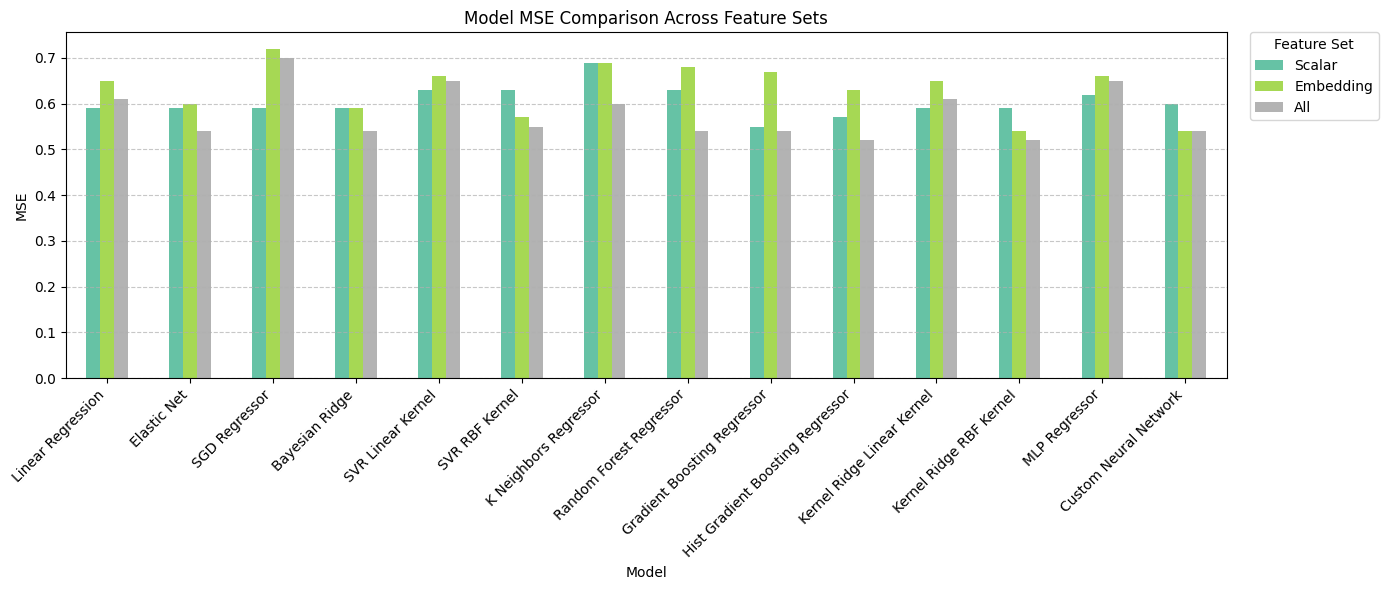
\includegraphics[width=1\linewidth]{images/mse_barplot.png}\hfill
    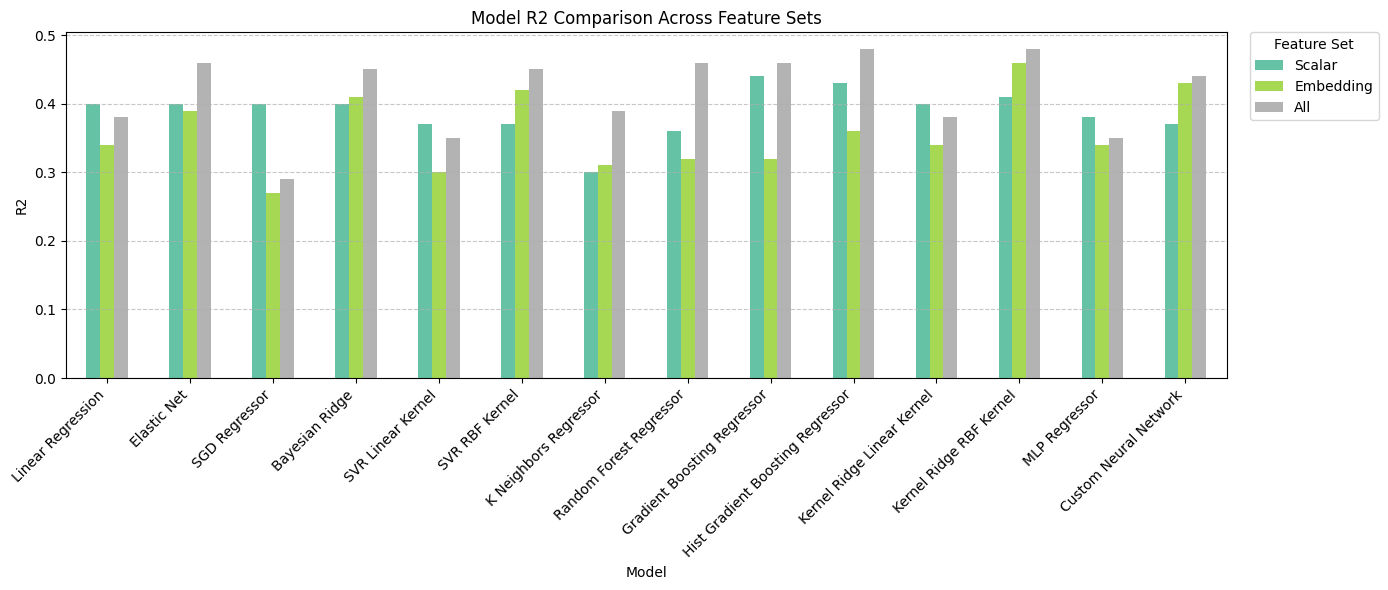
\includegraphics[width=1\linewidth]{images/r2_barplot.png}\hfill
    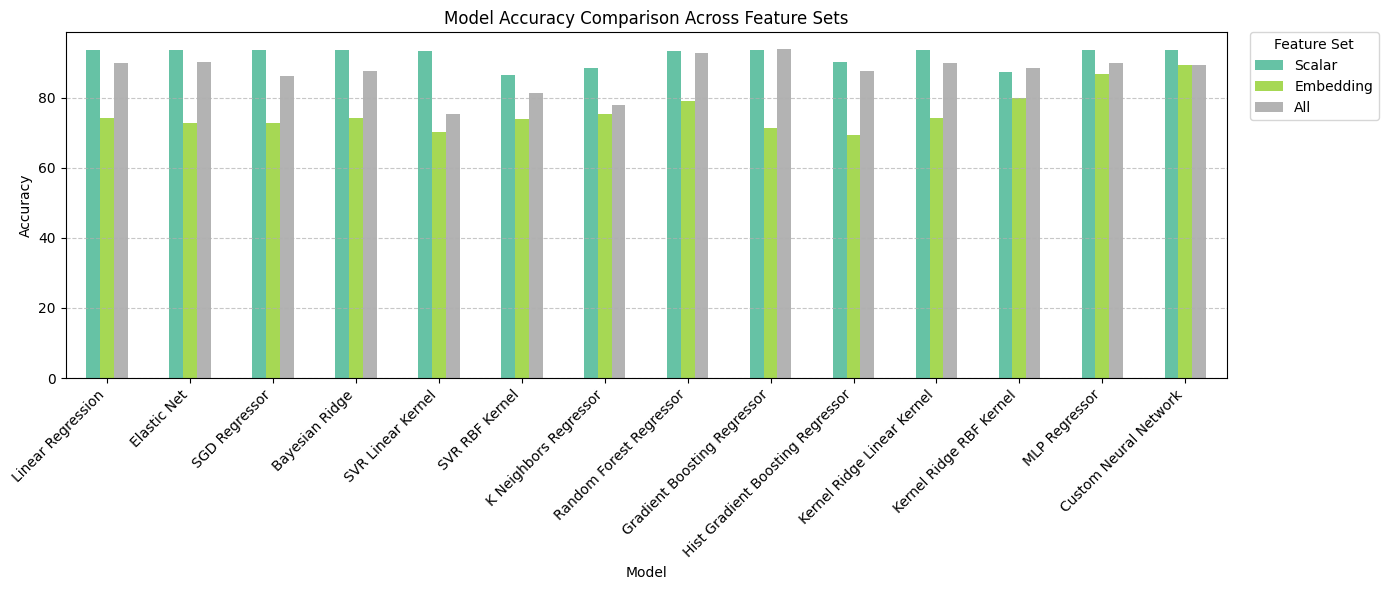
\includegraphics[width=1\linewidth]{images/accuracy_barplot.png}
    \caption{Bar-plots of MSE, $R^2$, and accuracy for the simple models.}
    \label{fig:simple_models_barplots}
\end{figure}


\section{BERT fine-tuning}
I also fine-tuned a BERT model for the task of predicting the total reading time for each word.

\subsection{Data Preparation}
The first step was to prepare the data for fine-tuning the BERT model. Since BERT works with tokenized input, in order to use the context, I organized the data by sentences. I created a dictionary where the keys are the sentence ids and the values are the sentence text, the list of words in the sentence, and the total reading time for each word in the sentence, which I used to create a dataframe. I then split the data into train, validation, and test sets, with 80\% of the data used for training, 10\% for validation, and 10\% for testing, and standardized the total reading time. The train set contains 250 sentences, while the validation and test sets contain 25 sentences each. The sentences were selected randomly.

Based on the dataframe, I created a dataset class built on the PyTorch Dataset class. The dataset class takes as input the dataframe, the tokenizer, and a maximum sequence length. It tokenizez the words in the sentences and creates the input tensors for the BERT model. It shortens the sentences to the maximum sequence length, and pads them if they are shorter than the maximum sequence length. The input tensors include the input ids, which are the tokenized words, the attention masks, which indicate which tokens are padding and which are not, and the targets, which are the total reading time for each word in the sentence. Because some words are split into multiple tokens, I used the word's reading time as the target for all tokens of the word.

\subsection{Model Architecture}
The first model I tried was BertForTokenClassification, using the pretrained \textit{dumitrescustefan/bert-base-romanian-uncased-v1} model, which I modified for a regression task. BertForTokenClassification is a BERT model with a linear layer on top that outputs the probabilities for each class. In this case, I used the logits from the output, which are the raw scores for each token before being passed through a softmax function, and set the number of output classes to 1, since I want to predict a single value (the total reading time) for each token. 

The second model I tried was a normal BERT model, also using the pretrained \textit{dumitrescustefan/bert-base-romanian-uncased-v1} model. On top of the BERT model, I added a regression head, which contains a linear layer, followed by ReLU activation, layer normalization and dropout, then another linear layer that outputs a single value (the total reading time). 

\subsection{Training}
I tried several different training strategies for the BERT models. The first strategy I tried was to simply train the whole model. Next, I tried various strategies based on gradual unfreezing, where I tried different numbers of layers to unfreeze every different number of epochs.

The strategy that worked best for the first model was training for a total of 30 epochs in 3 phases: the first 10 epochs with only the first 4 layers of BERT unfrozen, the next 10 epochs with the first 8 layers unfrozen, and the last 10 epochs with all layers unfrozen. I used the AdamW optimizer with a learning rate of 1e-4, a weight decay of 1e-4, and a cosine scheduler with warmup with 10 warmup steps. The batch size was set to 8, and the dropout rate was set to 0.3.

The strategy for the second model was based on gradual unfreezing: I first trained only the regression head for 5 epochs, then I gradually unfreezed the BERT layers, unfreezing 2 layers every 5 epochs, for a total of 35 epochs. I used the AdamW optimizer with a learning rate of 1e-4, a weight decay of 1e-4, and a cosine scheduler with warmup with 10 warmup steps. The batch size was set to 8, and the dropout rate was set to 0.3.

The loss function used for training was the mean squared error, which I customized to ignore the padding tokens in the input. For getting the word-level predictions, I averaged the predictions for each word based on the tokens that make up the word, so that the final prediction for each word is the average of the predictions for the tokens. The evaluation metrics were calculated on the word-level predictions.

\subsection{Results}
The results of the BERT fine-tuning models are shown in Table \ref{tab:bert_finetuning_results}.

\begin{table}
    \centering
    \begin{tabular}{|l|c|c|c|c|c|}
        \hline
        Model & MSE & R2 & Pearson & Spearman & Accuracy \\
        \hline
        BertForTokenClassification & 0.87 & 0.46 & 0.68 & 0.72 & 89.77 \\
        Bert with Regression Head & 0.88 & 0.45 & 0.67 & 0.73 & 89.65 \\
        \hline
    \end{tabular}
    \caption{Results of BERT fine-tuning models.}
    \label{tab:bert_finetuning_results}
\end{table}


\section{Leave-One-Out}
After training the models on randomly selected sentences from all the stimuli in the datatset, I also tried a leave-one-out strategy. Since the goal of the models is to predict the reading time for words in texts that were not seen during training, I selected some of the models and trained them on all stimuli except one, which was used for testing. I did this for each of the stimuli to see how well the models are capable to predict the reading time for texts that had no sentences seen during training.